\begin{figure}[htbp]
\section*{ SEC61A1}
\centering
\begin{subfigure}[b]{0.95\textwidth}
\centering
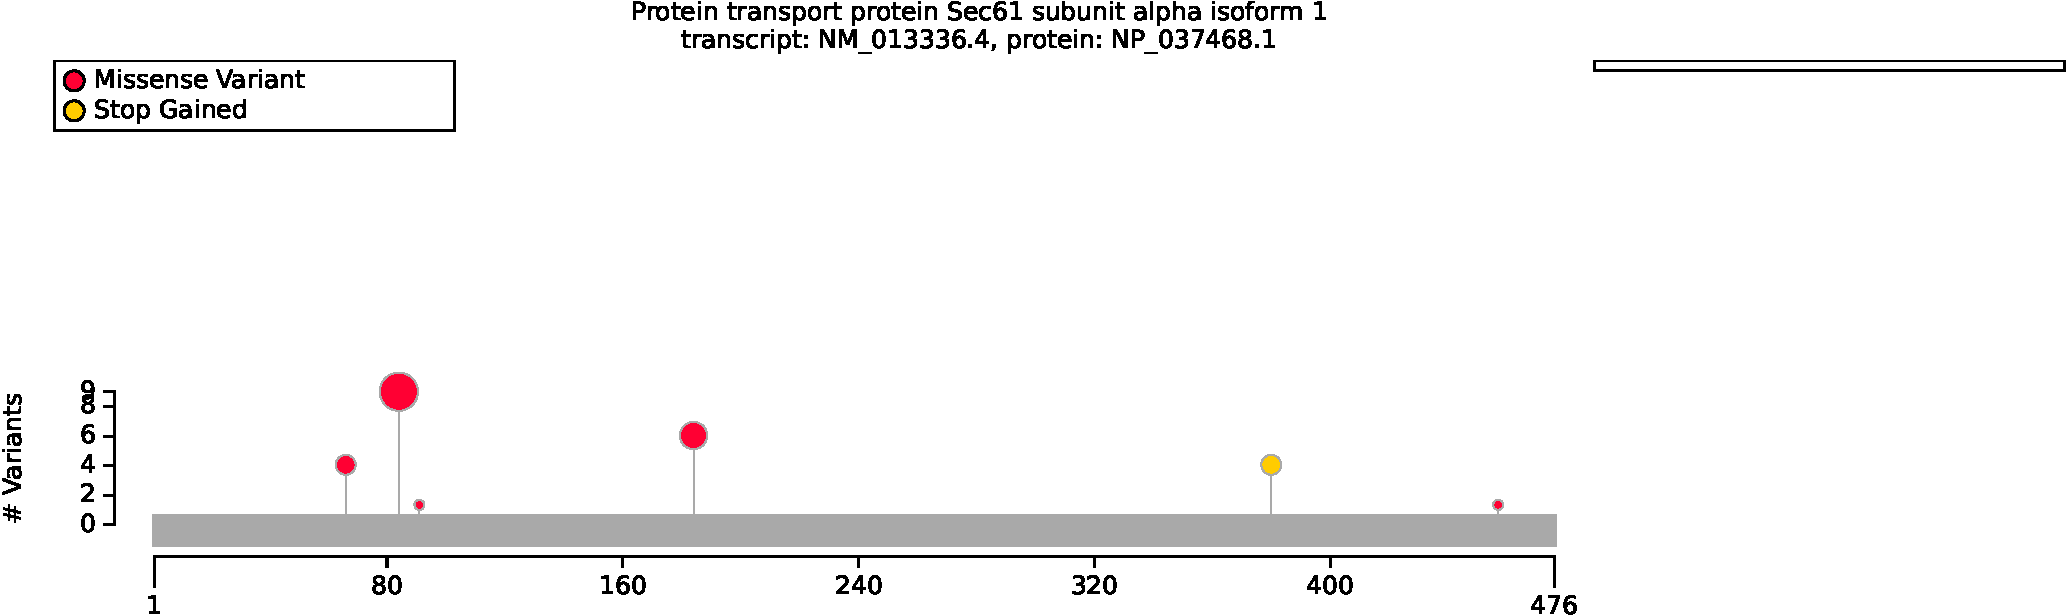
\includegraphics[width=\textwidth]{ img/SEC61A1_protein_diagram.pdf} 
\captionsetup{justification=raggedright,singlelinecheck=false}
\caption{Distribution of variants in SEC61A1}
\end{subfigure}

\vspace{2em}

\begin{subfigure}[b]{0.95\textwidth}
\centering
\resizebox{\textwidth}{!}{
\begin{tabular}{llllrr}
\toprule
Genotype (A) & Genotype (B) & total tests performed & significant results\\
\midrule
p.Val85Asp & Other variant & 24 & 0\\
FEMALE & MALE & 30 & 0\\
\bottomrule
\end{tabular}
}
\captionsetup{justification=raggedright,singlelinecheck=false}
\caption{             Fisher Exact Test performed to compare HPO annotation frequency with respect to genotypes. }
\end{subfigure}

\vspace{2em}

\caption{ The cohort comprised 19 individuals (8 females, 11 males). 1 of these individuals were reported to be deceased. A total of 76 HPO terms were used to annotate the cohort. Disease diagnoses: Immunodeficiency, common variable, 15 (OMIM:620670) (11 individuals), Tubulointerstitial kidney disease, autosomal dominant, 5 (OMIM:617056) (7 individuals), Neutropenia, severe congenital, 11, autosomal dominant (OMIM:620674) (1 individuals). The origin of clinical diversity in patients with SEC61A1 mutation is currently unclear. 
With our present patient set, a particular phenotype cannot be predicted on the basis of location or nature of the mutation \cite{PMID_32325141}.
 A total of 6 unique variant alleles were found in \textit{SEC61A1} (transcript: \texttt{NM\_013336.4}, protein id: \texttt{NP\_037468.1}).}
\end{figure}
